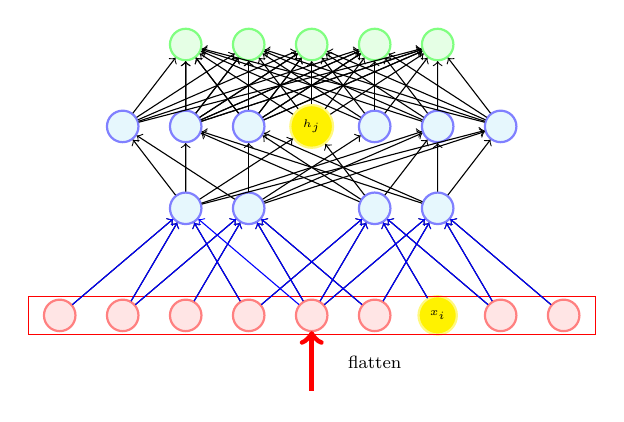
\begin{tikzpicture}[scale=0.8,transform shape]

	\tikzstyle{input_neuron}=[circle,draw=red!50,fill=red!10,thick,minimum size=5mm]
	\tikzstyle{input_neuron1}=[circle,draw=yellow!50,fill=yellow,thick,minimum size=5mm]
	\tikzstyle{hidden_neuron}=[circle,draw=blue!50,fill=cyan!10,thick,minimum size=5mm]
	\tikzstyle{hidden_neuron1}=[circle,draw=yellow!50,fill=yellow,thick,minimum size=5mm]
	\tikzstyle{output_neuron}=[circle,draw=green!50,fill=green!10,thick,minimum size=5mm]
	\tikzstyle{bias_neuron}=[circle,draw=red!50,fill=red!10,thick,minimum size=2mm]
	\tikzstyle{bias_hidden_neuron}=[circle,draw=blue!50,fill=cyan!10,thick,minimum size=2mm]
	\tikzstyle{bias_hidden_neuron_hi}=[circle,draw=orange,fill=cyan!10,thick,minimum size=2mm]
	\tikzstyle{bias_hidden_neuron_hi_old}=[circle,draw=yellow,fill=cyan!10,thick,minimum size=2mm]
	\tikzstyle{input}=[circle,draw=black!50,fill=black!20,thick,minimum size=6mm]
	
	\node [input_neuron] (B) at (-4.0,1){};
	\node [input_neuron] (C) at (-3,1){};
	\node [input_neuron] (D) at (-2,1){};
	\node [input_neuron] (E) at (-1,1){};
	\node [input_neuron] (F) at (0,1){};
	\node [input_neuron] (G) at (1,1){};
	\node [input_neuron1] (H) at (2,1){\tiny $x_i$};
	\node [input_neuron] (I) at (3,1){};
	\node [input_neuron] (J) at (4,1){};
	
	
	\node [rectangle, draw=red, minimum width=90mm, minimum height=6mm] at (0,1){};
	\node [hidden_neuron] (O) at (2,2.7){};
	\node [hidden_neuron] (N) at (1,2.7){};
	\node [hidden_neuron] (M) at (-1,2.7){};
	\node [hidden_neuron] (L) at (-2,2.7){};
	
	
	\node [hidden_neuron] (Oo) at (-3,4){};
	\node [hidden_neuron] (Nn) at (-2,4){};
	\node [hidden_neuron] (Mm) at (-1,4){};
	\node [hidden_neuron1] (Zz) at (0,4){\tiny $h_j$};
	
	\node [hidden_neuron] (Ll) at (1,4){};
	\node [hidden_neuron] (Xx) at (2,4){};
	\node [hidden_neuron] (Yy) at (3,4){};
	
	\node [output_neuron] (To) at (2,5.3){};
	\node [output_neuron] (Tp) at (1,5.3){};
	\node [output_neuron] (Tq) at (0,5.3){};
	\node [output_neuron] (Tr) at (-1,5.3){};
	\node [output_neuron] (Ts) at (-2,5.3){};
	\onslide<1->{
		
		\draw [->] (B) -- (L);
		\draw [->] (C) -- (L);
	
		\draw [->] (E) -- (L);
	
	
	
	
		\draw [->] (C) -- (M);
		\draw [->] (D) -- (M);
	
		\draw [->] (F) -- (M);
		\draw [->] (G) -- (M);
		\draw [->] (E) -- (N);
		\draw [->] (F) -- (N);
		\draw [->] (H) -- (N);
		\draw [->] (I) -- (N);
	
	
		\draw [->] (F) -- (O);
		\draw [->] (G) -- (O);
		\draw [->] (I) -- (O);
		\draw [->] (J) -- (O);
	
		\draw [->] (L) -- (Oo);
		
		\draw [->] (L) -- (Nn);	
		
		\draw [->] (L) -- (Xx);
		\draw [->] (L) -- (Yy);
		\draw [->] (L) -- (Zz);
	
	
	
		\draw [->] (M) -- (Oo);
		\draw [->] (M) -- (Mm);	
		
		\draw [->] (M) -- (Ll);
		\draw [->] (M) -- (Xx);
		\draw [->] (M) -- (Yy);
		
	
	
	
		
		\draw [->] (N) -- (Mm);	
		\draw [->] (N) -- (Nn);	
		
		\draw [->] (N) -- (Xx);
		
		\draw [->] (N) -- (Zz);
	
	
	
		
		\draw [->] (O) -- (Mm);	
		\draw [->] (O) -- (Nn);	
		
		\draw [->] (O) -- (Xx);
		\draw [->] (O) -- (Yy);
		
		\draw [->] (Ll) -- (To);
		\draw [->] (Ll) -- (Tp);
		\draw [->] (Ll) -- (Tq);
		\draw [->] (Ll) -- (Tr);
		\draw [->] (Ll) -- (Ts);
	
	
		\draw [->] (Mm) -- (To);
		\draw [->] (Mm) -- (Tp);
		\draw [->] (Mm) -- (Tq);
		\draw [->] (Mm) -- (Tr);
		\draw [->] (Mm) -- (Ts);
	
		\draw [->] (Nn) -- (To);
		\draw [->] (Nn) -- (Tp);
		\draw [->] (Nn) -- (Tq);
		\draw [->] (Nn) -- (Tr);
		\draw [->] (Nn) -- (Ts);
	
		\draw [->] (Mm) -- (To);
		\draw [->] (Mm) -- (Tp);
		\draw [->] (Mm) -- (Tq);
		\draw [->] (Mm) -- (Tr);
		\draw [->] (Mm) -- (Ts);
	
		\draw [->] (Nn) -- (To);
		\draw [->] (Nn) -- (Tp);
		\draw [->] (Nn) -- (Tq);
		\draw [->] (Nn) -- (Tr);
		\draw [->] (Nn) -- (Ts);
	
	
		\draw [->] (Oo) -- (To);
		\draw [->] (Oo) -- (Tp);
		\draw [->] (Oo) -- (Tq);
		\draw [->] (Oo) -- (Tr);
		\draw [->] (Oo) -- (Ts);
	
		\draw [->] (Xx) -- (To);
		\draw [->] (Xx) -- (Tp);
		\draw [->] (Xx) -- (Tq);
		\draw [->] (Xx) -- (Tr);
		\draw [->] (Xx) -- (Ts);
	
		\draw [->] (Yy) -- (To);
		\draw [->] (Yy) -- (Tp);
		\draw [->] (Yy) -- (Tq);
		\draw [->] (Yy) -- (Tr);
		\draw [->] (Yy) -- (Ts);
	
	
	
		\draw [->] (Zz) -- (To);
		\draw [->] (Zz) -- (Tp);
		\draw [->] (Zz) -- (Tq);
		\draw [->] (Zz) -- (Tr);
		\draw [->] (Zz) -- (Ts);
	
		\draw [->, line width=2, color=red] (0,-0.2)-- (0,0.75);
		\node [] at (1,0.25){\footnotesize flatten};
	}
	\onslide<1->{
		
		\draw [->,color=blue] (B) -- (L);
		\draw [->,color=blue] (C) -- (L);
	
		\draw [->,color=blue] (E) -- (L);
		\draw [->,color=blue] (F) -- (L);
	
	}
	
	\onslide<1->{
		
		\draw [->,color=blue] (C) -- (M);
		\draw [->,color=blue] (D) -- (M);
	
		\draw [->,color=blue] (F) -- (M);
		\draw [->,color=blue] (G) -- (M);
	}
	
	\onslide<1->{
		
		\draw [->,color=blue] (E) -- (N);
		\draw [->,color=blue] (F) -- (N);
	
		\draw [->,color=blue] (H) -- (N);
		\draw [->,color=blue] (I) -- (N);
	
	
	}
	
	\onslide<1->{
		
		\draw [->,color=blue] (F) -- (O);
		\draw [->,color=blue] (I) -- (O);
	
		\draw [->,color=blue] (G) -- (O);
		\draw [->,color=blue] (J) -- (O);
	
	
	}
\end{tikzpicture}

